\documentclass[10pt,sigconf,anonymous]{acmart}

\settopmatter{printacmref=true, printccs=false, printfolios=true}

\usepackage{booktabs} % For formal tables

\graphicspath{{figure/}{figures/}{Figure/}{Figures/}}

%% ------------------------------------------------------------------------------%
%% Miscelaneous packages
%% ------------------------------------------------------------------------------%

\usepackage{xspace}

%% ------------------------------------------------------------------------------%
%% Colors
%% ------------------------------------------------------------------------------%

\definecolor{backcolour}{rgb}{0.95,0.95,0.92}
\definecolor{bluekeywords}{rgb}{0.13,0.13,1}
\definecolor{codegray}{gray}{0.9}
\definecolor{ForestGreen}{RGB}{0,200,0}
\definecolor{mygreen}{rgb}{0,0.6,0}
\definecolor{mygray}{rgb}{0.5,0.5,0.5}
\definecolor{mymauve}{rgb}{0.58,0,0.82}
\definecolor{myteal}{RGB}{0,115,115}
\definecolor{redstrings}{rgb}{0.9,0,0}

%% ------------------------------------------------------------------------------%
%% Glossary
%% ------------------------------------------------------------------------------%

%% \usepackage[style=long3colheaderborder,acronym,automake,footnote,toc]{glossaries}
%% https://www.dickimaw-books.com/gallery/index.php?label=mixed-glossary-emph2
%% style=tree, stylemods=mcols
% \usepackage[automake,stylemods=mcols,toc]{glossaries-extra}
\usepackage[automake]{glossaries-extra}
% \newglossary[slg]{symbol}{sym}{sdn}{List of Symbols}
\makeglossaries
\setabbreviationstyle[acronym]{long-postshort-user}
\setabbreviationstyle[slg]{long-postshort-user}
%% Other styles are:
%% \setabbreviationstyle[acronym]{short-sc-postfootnote}
%% \setabbreviationstyle[acronym]{long-em-short-em}
%% \setabbreviationstyle[acronym]{short-footnote}
%% \setabbreviationstyle[acronym]{long-short-user}

% \renewcommand*{\glsfirstlonguserfont}[1]{\emph{#1}}
% \renewcommand{\glsxtrregularfont}[1]{\textcolor{violet}{\glsxtrifwasfirstuse{{#1}}{#1}}}
% \renewcommand{\glsxtrabbreviationfont}[1]{\textcolor{myteal}{\glsxtrifwasfirstuse{{#1}}{\texttt{#1}}}}
% \renewcommand{\glsxtrabbreviationfont}[1]{\textcolor{myteal}{\glsxtrifwasfirstuse{}{\let\glsfirstlonguserfont\glslonguserfont}#1}}
% \renewcommand{\glsxtrabbreviationfont}[1]{\textcolor{myteal}{\glsxtrifwasfirstuse{{{\let\glsfirstlonguserfont\glslonguserfont}#1}}{\texttt{#1}}}}

\renewcommand{\glsxtrregularfont}[1]{\textcolor{violet}{\glsxtrifwasfirstuse{{#1}}{#1}}}
\renewcommand{\glsxtrabbreviationfont}[1]{\textcolor{myteal}{\glsxtrifwasfirstuse{{#1}}{\texttt{#1}}}}

\renewcommand{\glsfirstabbrvuserfont}[1]{\textcolor{myteal}{\texttt{#1}}}

\renewcommand*{\glsxtrsetupfulldefs}{%
  \renewcommand*{\glsxtrifwasfirstuse}[2]{##2}%
}

%% ------------------------------------------------------------------------------%
%% Declare If Statements for Optional Pages
%% ------------------------------------------------------------------------------%

\newif\ifPageFigures
\newif\ifPageTables
\newif\ifPageGlossaries
\newif\ifPageContents
\newif\ifPageCodeSnippets
\newif\ifPageEquations

%% ------------------------------------------------------------------------------%
%% Set Default States for Optional Pages
%% ------------------------------------------------------------------------------%
\PageFiguresfalse
\PageTablesfalse
\PageGlossariesfalse
\PageContentsfalse
\PageCodeSnippetsfalse
\PageEquationsfalse

%% ------------------------------------------------------------------------------%
%% Command definitions
%% ------------------------------------------------------------------------------%

\definecolor{codegray}{gray}{0.9}
\newcommand{\code}[1]{\colorbox{codegray}{\texttt{#1}}}

%% ------------------------------------------------------------------------------%
%% Macros
%% ------------------------------------------------------------------------------%

% MPI Functions
\def\allreduce{\code{MPI\_Allreduce}\xspace}
\def\alltoall{\code{MPI\_Alltoall}\xspace}
\def\allgather{\code{MPI\_Allgather}\xspace}
\def\allgatherv{\code{MPI\_Allgatherv}\xspace}
\def\anysource{\code{MPI\_ANY\_SOURCE}\xspace}
\def\anytag{\code{MPI\_ANY\_TAG}\xspace}
\def\band{\code{MPI\_BAND}\xspace}
\def\barrier{\code{MPI\_Barrier}\xspace}
\def\bcast{\code{MPI\_Bcast}\xspace}
\def\comm{\emph{communicator}\xspace}
\def\finalize{\code{MPI\_Finalize}\xspace}
\def\gather{\code{MPI\_Gather}\xspace}
\def\gatherv{\code{MPI\_Gatherv}\xspace}
\def\iallgather{\code{MPI\_Iallgather}\xspace}
\def\iallreduce{\code{MPI\_Iallreduce}\xspace}
\def\id{\emph{id}\xspace}
\def\initthread{\code{MPI\_Init\_thread}\xspace}
\def\irecv{\code{MPI\_Irecv}\xspace}
\def\isend{\code{MPI\_Isend}\xspace}
\def\longlongint{\code{MPI\_LONG\_LONG\_INT}\xspace}
\def\mpit{\code{MPI\_T}\xspace}
\def\pmpi{\texttt{PMPI}\xspace}
\def\rank{\emph{rank}\xspace}
\def\ranks{\emph{ranks}\xspace}
\def\recv{\code{MPI\_Recv}\xspace}
\def\reduce{\code{MPI\_Reduce}\xspace}
\def\root{\emph{root}\xspace}
\def\rsa{\gls{RSA}\xspace}
\def\scan{\code{MPI\_Scan}\xspace}
\def\scatter{\code{MPI\_Scatter}\xspace}
\def\send{\code{MPI\_Send}\xspace}
\def\tag{\emph{tag}\xspace}
\def\threadsingle{\code{MPI\_THREAD\_SINGLE}\xspace}
\def\threadfunneled{\code{MPI\_THREAD\_FUNNELED}\xspace}
\def\threadmultiple{\code{MPI\_THREAD\_MULTIPLE}\xspace}
\def\threadserialized{\code{MPI\_THREAD\_SERIALIZED}\xspace}
\def\threadult{\code{MPI\_THREAD\_ULT}\xspace}
\def\wait{\code{MPI\_Wait}\xspace}
\def\waitall{\code{MPI\_Waitall}\xspace}
\def\waitany{\code{MPI\_Waitany}\xspace}
\def\win{\code{MPI\_Win}\xspace}

% Programming models, libraries, frameworks, technologies, algorithms, etc.
\def\algbinary{\emph{Binary}\xspace}
\def\algbinomial{\emph{Binomial}\xspace}
\def\algchain{\emph{Chain}\xspace}
\def\algknomial{\emph{Knomial}\xspace}
\def\alglinear{\emph{Linear}\xspace}
\def\algring{\emph{Ring}\xspace}
\def\algrsa{\gls{RSA}\xspace}
\def\algpairwise{\emph{Pairwise Exchange}\xspace}
\def\algpipeline{\emph{Pipeline}\xspace}
\def\algrab{\emph{Rabenseifner}\xspace}
\def\algrd{\emph{Recursive Doubling}\xspace}
\def\algrh{\emph{Recursive Halving}\xspace}
\def\algsegring{\emph{Segmented Ring}\xspace}
\def\algsynclinear{\emph{Synchornized Linear}\xspace}
\def\algtwoprocs{\emph{Two Processes}\xspace}
\def\api{\gls{API}\xspace}
\def\apis{\gls{API}s\xspace}
\def\beluga{B\'eluga\xspace}
\def\btl{\gls{BTL}\xspace}
\def\coll{\emph{collective}\xspace}
\def\Coll{\emph{Collective}\xspace}
\def\colls{\emph{collectives}\xspace}
\def\Colls{\emph{Collectives}\xspace}
\def\cntk{CNTK\xspace}
\def\cpu{\texttt{CPU}\xspace}
\def\cpus{\texttt{CPUs}\xspace}
\def\cuda{\gls{CUDA}\xspace}
\def\dl{\gls{DL}\xspace}
\def\dst{\emph{dst}\xspace}
\def\git{\texttt{git}\xspace}
\def\github{\texttt{GitHub}\xspace}
\def\google{\texttt{Google}\xspace}
\def\grep{\code{grep}\xspace}
\def\hct{\code{HOROVOD\_CYCLE\_TIME}\xspace}
\def\hpc{\gls{HPC}\xspace}
\def\hft{\code{HOROVOD\_FUSION\_THRESHOLD}\xspace}
\def\horovod{\texttt{Horovod}\xspace}
\def\ib{\gls{IB}\xspace}
\def\ipc{\gls{IPC}\xspace}
\def\ipcs{\gls{IPC}s\xspace}
\def\hashmap{\emph{HashMap}\xspace}
\def\keras{Keras\xspace}
\def\key{\emph{key}\xspace}
\def\linux{GNU/Linux\xspace}
\def\matex{MaTEx\xspace}
\def\msg{\emph{message matching}\xspace}
\def\Msg{\emph{Message matching}\xspace}
\def\ml{Machine Learning\xspace}
\def\mpi{\gls{MPI}\xspace}
\def\mpich{\texttt{MPICH}\xspace}
\def\mpichucx{\texttt{MPICH+}\gls{UCX}\xspace}
\def\mpicuda{\gls{MPI}\texttt{+}\gls{CUDA}\xspace}
\def\mpimpi{\gls{MPI}\texttt{+}\gls{MPI}\xspace}
\def\mpinccl{\gls{MPI}\texttt{+}\gls{NCCL}\xspace}
\def\mpiopencl{\gls{MPI}\texttt{+}\gls{OpenCL}\xspace}
\def\mpithree{\gls{MPI}\texttt{-3}\xspace}
\def\mpix{\gls{MPI}\texttt{+X}\xspace}
\def\mvapich{\texttt{MVAPICH}\xspace}
\def\mvapichtwo{\texttt{MVAPICH2}\xspace}
\def\mvapichtwogdr{\texttt{MVAPICH2-}\gls{GDR}\xspace}
\def\mxnet{MXNet\xspace}
\def\nic{\gls{NIC}\xspace}
\def\nics{\gls{NIC}\texttt{s}\xspace}
\def\nccl{\gls{NCCL}\xspace}
\def\ncclrecv{\code{NCCL\_Recv}\xspace}
\def\ncclsend{\code{NCCL\_Send}\xspace}
\def\nccltwo{\gls{NCCL}\texttt{2}\xspace}
\def\omp{\gls{OpenMP}\xspace}
\def\ompi{\gls{OMPI}\xspace}
\def\opal{\gls{OPAL}\xspace}
\def\opencl{\gls{OpenCL}\xspace}
\def\openacc{\gls{OpenACC}\xspace}
\def\openmpi{\texttt{Open }\gls{MPI}\xspace}
\def\openmpiucx{\texttt{Open }\gls{MPI}+\gls{UCX}\xspace}
\def\openshmem{\gls{OpenSHMEM}\xspace}
\def\os{\gls{OS}\xspace}
\def\osc{\emph{one-sided}\xspace}
\def\Osc{\emph{One-sided}\xspace}
\def\pap{\gls{PAP}\xspace}
\def\paps{\gls{PAP}s\xspace}
\def\part{\emph{partitioned}\xspace}
\def\pat{\gls{PAT}\xspace}
\def\pats{\gls{PAT}s\xspace}
\def\prrte{\gls{PRRTE}\xspace}
\def\pt{PyTorch\xspace}
\def\pthreads{\gls{Pthreads}\xspace}
\def\ptp{\gls{P2P}\xspace}
\def\ptps{\gls{P2P}s\xspace}
\def\rl{Reinforcement Learning\xspace}
\def\sharp{SHARP\texttrademark\xspace}
\def\systemv{\texttt{System V}\xspace}
\def\src{\emph{src}\xspace}
\def\tf{\texttt{TensorFlow}\xspace}
\def\tfbench{\code{tf\_cnn\_benchmark}\xspace}
\def\temp{\emph{temp}\xspace}
\def\ucc{\gls{UCC}\xspace}
\def\ucf{\gls{UCF}\xspace}
\def\ucp{\gls{UCP}\xspace}
\def\ucs{\gls{UCS}\xspace}
\def\uct{\gls{UCT}\xspace}
\def\ucx{\gls{UCX}\xspace}

% GPUs, CUDA, & NVIDIA
\def\asynccopy{\gls{AC}\xspace}
\def\amd{\texttt{AMD}\xspace}
\def\ampere{\texttt{Ampere}\xspace}
\def\cgroups{\texttt{Cooperative Groups}\xspace}
\def\cgraph{\gls{CUDA} \texttt{Graph}\xspace}
\def\cgraphs{\gls{CUDA} \texttt{Graphs}\xspace}
\def\cstream{\gls{CUDA} \texttt{stream}\xspace}
\def\cstreams{\gls{CUDA} \texttt{streams}\xspace}
\def\cudadevsync{\code{cudaDeviceSynchronize}\xspace}
\def\cudamemadvise{\code{cudaMemAdvise}\xspace}
\def\cudamemcpy{\code{cudaMemcpy}\xspace}
\def\cudamemcpyasync{\code{cudaMemcpyAsync}\xspace}
\def\cudamemset{\code{cudaMemset}\xspace}
\def\cudamemprefetch{\code{cudaMemPrefetch}\xspace}
\def\cudastreamsync{\code{cudaStreamSynchronize}\xspace}
\def\dgxone{\texttt{DGX-1}\xspace}
\def\dgxtwo{\texttt{DGX-2}\xspace}
\def\event{\emph{event}\xspace}
\def\events{\emph{events}\xspace}
%\def\gpudirect{GPUDirect\textsuperscript{\textregistered}\xspace}
\def\gdr{\gls{GDR}\xspace}
\def\gpu{\gls{GPU}\xspace}
\def\gpus{\gls{GPU}s\xspace}
\def\gpudirect{\texttt{GPUDirect}\xspace}
\def\gpudirectptp{\texttt{GPUDirect\_}\gls{P2P}\xspace}
\def\gpudirectasync{\texttt{GPUDirect\_Async}\xspace}
\def\gpudirectrdma{\texttt{GPUDirect\_}\gls{RDMA}\xspace}
\def\graphlaunch{\code{cudaGraphLaunch}\xspace}
\def\gstream{\gls{GPU} \texttt{stream}\xspace}
\def\gstreams{\gls{GPU} \texttt{streams}\xspace}
\def\host{\emph{host}\xspace}
\def\hyperq{\texttt{Hyper-Q}\xspace}
\def\kernel{\texttt{kernel}\xspace}
\def\kernels{\texttt{kernels}\xspace}
\def\mellanox{\texttt{Mellanox}\xspace}
\def\mig{\gls{MIG}\xspace}
\def\mps{\gls{MPS}\xspace}
\def\nvidia{\texttt{NVIDIA}\xspace}
\def\nvgroup{\texttt{NVGroup}\xspace}
\def\nvlink{\texttt{NVLink}\xspace}
\def\nvlinkone{\texttt{NVLink-V1}\xspace}
\def\nvlinks{\texttt{NVLinks}\xspace}
\def\nvlinktwo{\texttt{NVLink-V2}\xspace}
\def\nvlinkthree{\texttt{NVLink-V3}\xspace}
\def\nvlinksli{\gls{NVLink-SLI}\xspace}
\def\nvswitch{\texttt{NVSwitch}\xspace}
\def\pcie{\gls{PCIe}\xspace}
\def\sm{\gls{SM}\xspace}
\def\sms{\gls{SM}s\xspace}
\def\stream{\texttt{stream}\xspace}
\def\streams{\texttt{streams}\xspace}
\def\volta{\texttt{Volta}\xspace}

% ACRONYMS
% \newacronym{NameInSort}{NameToShow}{Definition}
\newacronym{AC}{AC}{Asynchronous Copy}
\newacronym{ANL}{ANL}{Argonne National Laboratory}
\newacronym{ARMCI}{ARMCI}{Aggregate Remote Memory Copy Interface}
\newacronym{API}{API}{Application Programming Interface}
\newacronym{ATS}{ATS}{Address Translation Services}
\newacronym{BLAS}{BLAS}{Basic Linear Algebra Subprograms}
\newacronym{BTB}{BTB}{Binomial Tree Based}
\newacronym{BTL}{BTL}{Byte Transfer Layer}
\newacronym{BPMF}{BPMF}{Bayesian Probabilistic Matrix Factorize}
\newacronym{CHAMPION}{CHAMPION}{Communication-aware Hardware-Assisted MPI Overlap eNgine}
\newacronym{CISC}{CISC}{Complex Instruction Set Computing}
\newacronym{CNN}{CNN}{Convolutional Neural Networks}
\newacronym{CQ}{CQ}{Completion Queue}
\newacronym{CRI}{CRI}{Communication Resources Instance}
\newacronym{CTS}{CTS}{Clear To Send}
\newacronym{cuBLAS}{cuBLAS}{NVIDIA CUDA Blas Library}
\newacronym{CUDA}{CUDA}{Compute Unified Device Architecture}
\newacronym{CUDA-Capable}{CUDA-Capable}{Capable for programming in CUDA Platform}
\newacronym{cuFFT}{cuFFT}{NVIDIA CUDA Fast Fourier Transform Library}
\newacronym{cuDNN}{cuDNN}{NVIDIA CUDA Deep Neural Networks Library}
\newacronym{cuRAND}{cuRAND}{NVIDIA CUDA Random Number Generator Library}
\newacronym{cuSPARSE}{cuSPARSE}{NVIDIA CUDA Sparse Matrix Library}
\newacronym{DAG}{DAG}{Directed Acyclic Graph}
\newacronym{DL}{DL}{Deep Learning}
\newacronym{DMA}{DMA}{Direct Memory Access}
\newacronym{DNN}{DNN}{Deep Neural Networks}
\newacronym{DriverAPI}{Driver API}{Driver Application Programming Interface}
\newacronym{DSL}{DSL}{Domain-Specific Language}
\newacronym{EP}{EP}{Endpoints}
\newacronym{ETL}{ETL}{Extract, Transform and Load}
\newacronym{FDS}{FDS}{Fire Dynamics Simulator}
\newacronym{FLOPS}{FLOPS}{Floating-point Operations Per Second}
\newacronym{FFT}{FFT}{Fast Fourier Transform}
\newacronym{GCC}{GCC}{GNU Compiler Collection}
\newacronym{GDR}{GDR}{GPUDirect RDMA}
\newacronym{GPU}{GPU}{Graphics Processing Unit}
\newacronym{GPGPU}{GPGPU}{General Purpose Computing on Graphics Processing Unit}
\newacronym{GSB}{GSB}{GPU Shared Buffer}
\newacronym{HCA}{HCA}{Host Channel Adapter}
\newacronym{HDFS}{HDFS}{Hadoop File System}
\newacronym{HMCS}{HMCS}{Hierarchical MCS}
\newacronym{HMPI}{HMPI}{Hybrid MPI}
\newacronym{HOL}{HOL}{Head-Of-Line}
\newacronym{HOOMD-blue}{HOOMD-blue}{Highly Optimized Object-oriented Many-particle
	Dynamics - Blue Edition}
\newacronym{HPC}{HPC}{High-Performance Computing}
\newacronym{HPL}{HPL}{High-Performance Linpack}
\newacronym{IB}{IB}{InfiniBand}
\newacronym{IPC}{IPC}{Inter-Process Communication}
\newacronym{ILP}{ILP}{Instruction Level Parallelism}
\newacronym{ISA}{ISA}{Instruction Set Architecture}
\newacronym{IPO}{IPO}{Input Processor Output}
\newacronym{JCUDA}{JCUDA}{Java Bindings for CUDA}
\newacronym{JNI}{JNI}{Java Native Interface}
\newacronym{JVM}{JVM}{Java Virtual Machine}
\newacronym{LAMMPS}{LAMMPS}{Large-scale Atomic/Molecular Massively Parallel Simulator}
\newacronym{LBM}{LBM}{Lattice Boltzmann Method}
\newacronym{LLN}{LLN}{Low-Level Network}
\newacronym{LMT}{LMT}{Large Message Transfer}
\newacronym{MAGC}{MAGC}{Mapping Approach for GPU Clusters}
\newacronym{MCS}{MCS}{Mellor-Crummey and Scott}
\newacronym{MIG}{MIG}{Multi-Instance GPU}
\newacronym{MIPS}{MIPS}{Million Instructions Per Second}
\newacronym{MPI}{MPI}{Message Passing Interface}
\newacronym{MPP}{MPP}{Massively Parallel Processors}
\newacronym{MPS}{MPS}{Multi-Process Service}
\newacronym{MT-MPI}{MT-MPI}{Multi-Threaded MPI}
\newacronym{Mutex}{Mutex}{Mutual Exclusion}
\newacronym{NBC}{NBC}{Non-Blocking Collective}
\newacronym{NCCL}{NCCL}{NVIDIA Collective Communications Library}
\newacronym{NIC}{NIC}{Network Interface Card}
\newacronym{NPB}{NPB}{NAS Parallel Benchmark suit}
\newacronym{NUMA}{NUMA}{Non-Uniform Memory Access}
\newacronym{NVLink-SLI}{NVLink-SLI}{NVIDIA Scalable Link Interface}
\newacronym{OMB}{OMB}{OSU Micro-Benchmarks}
\newacronym{OMPI}{OMPI}{Open MPI}
\newacronym{OPAL}{OPAL}{Open Portable Access Layer}
\newacronym{OpenACC}{OpenACC}{Open Accelerators}
\newacronym{OpenCL}{OpenCL}{Open Computing Language}
\newacronym{OpenCV}{OpenCV}{Open Computer Vision}
\newacronym{OpenGL}{OpenGL}{Open Graphic Library}
\newacronym{OpenMP}{OpenMP}{Open Multi-Processing}
\newacronym{OpenSHMEM}{OpenSHMEM}{Open Symmetric Hierarchical MEMory}
\newacronym{OS}{OS}{Operating System}
\newacronym{OSC}{OSC}{One-Sided Communication}
\newacronym{P2P}{P2P}{Point-to-Point}
\newacronym{PAP}{PAP}{Process Arrival Pattern}
\newacronym{PAT}{PAT}{Process Arrival Time}
\newacronym{PCIe}{PCIe}{Peripheral Component Interconnect Express}
\newacronym{PGAS}{PGAS}{Partitioned Global Address Space}
\newacronym{PIE}{PIE}{Position-Independent Executables}
\newacronym{POSIX}{POSIX}{Portable Operating System Interface}
\newacronym{PRQ}{PRQ}{Posted Receive Queue}
\newacronym{PRRTE}{PRRTE}{Process Management Interface (PMIx) Reference RunTime Environment}
\newacronym{Pthreads}{Pthreads}{POSIX Threads}
\newacronym{PTX}{PTX}{Parallel Thread Execution}
\newacronym{QE}{QE}{Queue Element}
\newacronym{RAW}{RAW}{Read After Write}
\newacronym{RDMA}{RDMA}{Remote Direct Memory Access}
\newacronym{RMA}{RMA}{Remote Memory Access}
\newacronym{RISC}{RISC}{Reduced Instruction Set Computing}
\newacronym{RSA}{RSA}{Reduce Scatter Allgather}
\newacronym{RTS}{RTS}{Request To Send}
\newacronym{RuntimeAPI}{Runtime API}{Runtime Application Programming Interface}
\newacronym{SHOC}{SHOC}{Scalable Heterogeneous Computing benchmark suite}
\newacronym{SHM}{SHM}{Shared Memory}
\newacronym{SIMD}{SIMD}{Single Instruction Multiple Data}
\newacronym{SIMT}{SIMT}{Single Instruction Multiple Thread}
\newacronym{SM}{SM}{Streaming Multiprocessor}
\newacronym{SMP}{SMP}{Symmetric Multi-Processor}
\newacronym{SQL}{SQL}{Structured Query Language}
\newacronym{TGCS}{TGCS}{Task Graph Computing System}
\newacronym{UCC}{UCC}{Unified Communication Collectives}
\newacronym{UCF}{UCF}{Unified Communication Framework}
\newacronym{UCP}{UCP}{Unified Communication Protocols}
\newacronym{UCS}{UCS}{Unified Communication Services}
\newacronym{UCT}{UCT}{Unified Communication Transports}
\newacronym{UCX}{UCX}{Unified Communication X}
\newacronym{ULT}{ULT}{User-Level Threads}
\newacronym{UM}{UM}{Unified Memory}
\newacronym{UMQ}{UMQ}{Unexpected Message Queue}
\newacronym{UPC}{UPC}{Unified Parallel C}
\newacronym{UVA}{UVA}{Unified Virtual Addressing}
\newacronym{VAS}{VAS}{Virtual Address Space}
\newacronym{VLIW}{VLIW}{Very Long Instruction Word}
\newacronym{VNI}{VNI}{Virtual Network Interface}
\newacronym{WAR}{WAR}{Write After Read}
\newacronym{WAW}{WAW}{Write After Write}
\newacronym{YARN}{Apache YARN}{Yet Another Resource Negotiator}

%% ------------------------------------------------------------------------------%%% ------------------------------------------------------------------------------%
%% Miscelaneous packages
%% ------------------------------------------------------------------------------%

\usepackage{xspace}

%% ------------------------------------------------------------------------------%
%% Colors
%% ------------------------------------------------------------------------------%

\definecolor{backcolour}{rgb}{0.95,0.95,0.92}
\definecolor{bluekeywords}{rgb}{0.13,0.13,1}
\definecolor{codegray}{gray}{0.9}
\definecolor{ForestGreen}{RGB}{0,200,0}
\definecolor{mygreen}{rgb}{0,0.6,0}
\definecolor{mygray}{rgb}{0.5,0.5,0.5}
\definecolor{mymauve}{rgb}{0.58,0,0.82}
\definecolor{myteal}{RGB}{0,115,115}
\definecolor{redstrings}{rgb}{0.9,0,0}

%% ------------------------------------------------------------------------------%
%% Glossary
%% ------------------------------------------------------------------------------%

%% \usepackage[style=long3colheaderborder,acronym,automake,footnote,toc]{glossaries}
%% https://www.dickimaw-books.com/gallery/index.php?label=mixed-glossary-emph2
%% style=tree, stylemods=mcols
% \usepackage[automake,stylemods=mcols,toc]{glossaries-extra}
\usepackage[automake]{glossaries-extra}
% \newglossary[slg]{symbol}{sym}{sdn}{List of Symbols}
\makeglossaries
\setabbreviationstyle[acronym]{long-postshort-user}
\setabbreviationstyle[slg]{long-postshort-user}
%% Other styles are:
%% \setabbreviationstyle[acronym]{short-sc-postfootnote}
%% \setabbreviationstyle[acronym]{long-em-short-em}
%% \setabbreviationstyle[acronym]{short-footnote}
%% \setabbreviationstyle[acronym]{long-short-user}

% \renewcommand*{\glsfirstlonguserfont}[1]{\emph{#1}}
% \renewcommand{\glsxtrregularfont}[1]{\textcolor{violet}{\glsxtrifwasfirstuse{{#1}}{#1}}}
% \renewcommand{\glsxtrabbreviationfont}[1]{\textcolor{myteal}{\glsxtrifwasfirstuse{{#1}}{\texttt{#1}}}}
% \renewcommand{\glsxtrabbreviationfont}[1]{\textcolor{myteal}{\glsxtrifwasfirstuse{}{\let\glsfirstlonguserfont\glslonguserfont}#1}}
% \renewcommand{\glsxtrabbreviationfont}[1]{\textcolor{myteal}{\glsxtrifwasfirstuse{{{\let\glsfirstlonguserfont\glslonguserfont}#1}}{\texttt{#1}}}}

\renewcommand{\glsxtrregularfont}[1]{\textcolor{violet}{\glsxtrifwasfirstuse{{#1}}{#1}}}
\renewcommand{\glsxtrabbreviationfont}[1]{\textcolor{myteal}{\glsxtrifwasfirstuse{{#1}}{\texttt{#1}}}}

\renewcommand{\glsfirstabbrvuserfont}[1]{\textcolor{myteal}{\texttt{#1}}}

\renewcommand*{\glsxtrsetupfulldefs}{%
  \renewcommand*{\glsxtrifwasfirstuse}[2]{##2}%
}

%% ------------------------------------------------------------------------------%
%% Declare If Statements for Optional Pages
%% ------------------------------------------------------------------------------%

\newif\ifPageFigures
\newif\ifPageTables
\newif\ifPageGlossaries
\newif\ifPageContents
\newif\ifPageCodeSnippets
\newif\ifPageEquations

%% ------------------------------------------------------------------------------%
%% Set Default States for Optional Pages
%% ------------------------------------------------------------------------------%
\PageFiguresfalse
\PageTablesfalse
\PageGlossariesfalse
\PageContentsfalse
\PageCodeSnippetsfalse
\PageEquationsfalse

%% ------------------------------------------------------------------------------%
%% Command definitions
%% ------------------------------------------------------------------------------%

\definecolor{codegray}{gray}{0.9}
\newcommand{\code}[1]{\colorbox{codegray}{\texttt{#1}}}

%% ------------------------------------------------------------------------------%
%% Macros
%% ------------------------------------------------------------------------------%

% MPI Functions
\def\allreduce{\code{MPI\_Allreduce}\xspace}
\def\alltoall{\code{MPI\_Alltoall}\xspace}
\def\allgather{\code{MPI\_Allgather}\xspace}
\def\allgatherv{\code{MPI\_Allgatherv}\xspace}
\def\anysource{\code{MPI\_ANY\_SOURCE}\xspace}
\def\anytag{\code{MPI\_ANY\_TAG}\xspace}
\def\band{\code{MPI\_BAND}\xspace}
\def\barrier{\code{MPI\_Barrier}\xspace}
\def\bcast{\code{MPI\_Bcast}\xspace}
\def\comm{\emph{communicator}\xspace}
\def\finalize{\code{MPI\_Finalize}\xspace}
\def\gather{\code{MPI\_Gather}\xspace}
\def\gatherv{\code{MPI\_Gatherv}\xspace}
\def\iallgather{\code{MPI\_Iallgather}\xspace}
\def\iallreduce{\code{MPI\_Iallreduce}\xspace}
\def\id{\emph{id}\xspace}
\def\initthread{\code{MPI\_Init\_thread}\xspace}
\def\irecv{\code{MPI\_Irecv}\xspace}
\def\isend{\code{MPI\_Isend}\xspace}
\def\longlongint{\code{MPI\_LONG\_LONG\_INT}\xspace}
\def\mpit{\code{MPI\_T}\xspace}
\def\pmpi{\texttt{PMPI}\xspace}
\def\rank{\emph{rank}\xspace}
\def\ranks{\emph{ranks}\xspace}
\def\recv{\code{MPI\_Recv}\xspace}
\def\reduce{\code{MPI\_Reduce}\xspace}
\def\root{\emph{root}\xspace}
\def\rsa{\gls{RSA}\xspace}
\def\scan{\code{MPI\_Scan}\xspace}
\def\scatter{\code{MPI\_Scatter}\xspace}
\def\send{\code{MPI\_Send}\xspace}
\def\tag{\emph{tag}\xspace}
\def\threadsingle{\code{MPI\_THREAD\_SINGLE}\xspace}
\def\threadfunneled{\code{MPI\_THREAD\_FUNNELED}\xspace}
\def\threadmultiple{\code{MPI\_THREAD\_MULTIPLE}\xspace}
\def\threadserialized{\code{MPI\_THREAD\_SERIALIZED}\xspace}
\def\threadult{\code{MPI\_THREAD\_ULT}\xspace}
\def\wait{\code{MPI\_Wait}\xspace}
\def\waitall{\code{MPI\_Waitall}\xspace}
\def\waitany{\code{MPI\_Waitany}\xspace}
\def\win{\code{MPI\_Win}\xspace}

% Programming models, libraries, frameworks, technologies, algorithms, etc.
\def\algbinary{\emph{Binary}\xspace}
\def\algbinomial{\emph{Binomial}\xspace}
\def\algchain{\emph{Chain}\xspace}
\def\algknomial{\emph{Knomial}\xspace}
\def\alglinear{\emph{Linear}\xspace}
\def\algring{\emph{Ring}\xspace}
\def\algrsa{\gls{RSA}\xspace}
\def\algpairwise{\emph{Pairwise Exchange}\xspace}
\def\algpipeline{\emph{Pipeline}\xspace}
\def\algrab{\emph{Rabenseifner}\xspace}
\def\algrd{\emph{Recursive Doubling}\xspace}
\def\algrh{\emph{Recursive Halving}\xspace}
\def\algsegring{\emph{Segmented Ring}\xspace}
\def\algsynclinear{\emph{Synchornized Linear}\xspace}
\def\algtwoprocs{\emph{Two Processes}\xspace}
\def\api{\gls{API}\xspace}
\def\apis{\gls{API}s\xspace}
\def\beluga{B\'eluga\xspace}
\def\btl{\gls{BTL}\xspace}
\def\coll{\emph{collective}\xspace}
\def\Coll{\emph{Collective}\xspace}
\def\colls{\emph{collectives}\xspace}
\def\Colls{\emph{Collectives}\xspace}
\def\cntk{CNTK\xspace}
\def\cpu{\texttt{CPU}\xspace}
\def\cpus{\texttt{CPUs}\xspace}
\def\cuda{\gls{CUDA}\xspace}
\def\dl{\gls{DL}\xspace}
\def\dst{\emph{dst}\xspace}
\def\git{\texttt{git}\xspace}
\def\github{\texttt{GitHub}\xspace}
\def\google{\texttt{Google}\xspace}
\def\grep{\code{grep}\xspace}
\def\hct{\code{HOROVOD\_CYCLE\_TIME}\xspace}
\def\hpc{\gls{HPC}\xspace}
\def\hft{\code{HOROVOD\_FUSION\_THRESHOLD}\xspace}
\def\horovod{\texttt{Horovod}\xspace}
\def\ib{\gls{IB}\xspace}
\def\ipc{\gls{IPC}\xspace}
\def\ipcs{\gls{IPC}s\xspace}
\def\hashmap{\emph{HashMap}\xspace}
\def\keras{Keras\xspace}
\def\key{\emph{key}\xspace}
\def\linux{GNU/Linux\xspace}
\def\matex{MaTEx\xspace}
\def\msg{\emph{message matching}\xspace}
\def\Msg{\emph{Message matching}\xspace}
\def\ml{Machine Learning\xspace}
\def\mpi{\gls{MPI}\xspace}
\def\mpich{\texttt{MPICH}\xspace}
\def\mpichucx{\texttt{MPICH+}\gls{UCX}\xspace}
\def\mpicuda{\gls{MPI}\texttt{+}\gls{CUDA}\xspace}
\def\mpimpi{\gls{MPI}\texttt{+}\gls{MPI}\xspace}
\def\mpinccl{\gls{MPI}\texttt{+}\gls{NCCL}\xspace}
\def\mpiopencl{\gls{MPI}\texttt{+}\gls{OpenCL}\xspace}
\def\mpithree{\gls{MPI}\texttt{-3}\xspace}
\def\mpix{\gls{MPI}\texttt{+X}\xspace}
\def\mvapich{\texttt{MVAPICH}\xspace}
\def\mvapichtwo{\texttt{MVAPICH2}\xspace}
\def\mvapichtwogdr{\texttt{MVAPICH2-}\gls{GDR}\xspace}
\def\mxnet{MXNet\xspace}
\def\nic{\gls{NIC}\xspace}
\def\nics{\gls{NIC}\texttt{s}\xspace}
\def\nccl{\gls{NCCL}\xspace}
\def\ncclrecv{\code{NCCL\_Recv}\xspace}
\def\ncclsend{\code{NCCL\_Send}\xspace}
\def\nccltwo{\gls{NCCL}\texttt{2}\xspace}
\def\omp{\gls{OpenMP}\xspace}
\def\ompi{\gls{OMPI}\xspace}
\def\opal{\gls{OPAL}\xspace}
\def\opencl{\gls{OpenCL}\xspace}
\def\openacc{\gls{OpenACC}\xspace}
\def\openmpi{\texttt{Open }\gls{MPI}\xspace}
\def\openmpiucx{\texttt{Open }\gls{MPI}+\gls{UCX}\xspace}
\def\openshmem{\gls{OpenSHMEM}\xspace}
\def\os{\gls{OS}\xspace}
\def\osc{\emph{one-sided}\xspace}
\def\Osc{\emph{One-sided}\xspace}
\def\pap{\gls{PAP}\xspace}
\def\paps{\gls{PAP}s\xspace}
\def\part{\emph{partitioned}\xspace}
\def\pat{\gls{PAT}\xspace}
\def\pats{\gls{PAT}s\xspace}
\def\prrte{\gls{PRRTE}\xspace}
\def\pt{PyTorch\xspace}
\def\pthreads{\gls{Pthreads}\xspace}
\def\ptp{\gls{P2P}\xspace}
\def\ptps{\gls{P2P}s\xspace}
\def\rl{Reinforcement Learning\xspace}
\def\sharp{SHARP\texttrademark\xspace}
\def\systemv{\texttt{System V}\xspace}
\def\src{\emph{src}\xspace}
\def\tf{\texttt{TensorFlow}\xspace}
\def\tfbench{\code{tf\_cnn\_benchmark}\xspace}
\def\temp{\emph{temp}\xspace}
\def\ucc{\gls{UCC}\xspace}
\def\ucf{\gls{UCF}\xspace}
\def\ucp{\gls{UCP}\xspace}
\def\ucs{\gls{UCS}\xspace}
\def\uct{\gls{UCT}\xspace}
\def\ucx{\gls{UCX}\xspace}

% GPUs, CUDA, & NVIDIA
\def\asynccopy{\gls{AC}\xspace}
\def\amd{\texttt{AMD}\xspace}
\def\ampere{\texttt{Ampere}\xspace}
\def\cgroups{\texttt{Cooperative Groups}\xspace}
\def\cgraph{\gls{CUDA} \texttt{Graph}\xspace}
\def\cgraphs{\gls{CUDA} \texttt{Graphs}\xspace}
\def\cstream{\gls{CUDA} \texttt{stream}\xspace}
\def\cstreams{\gls{CUDA} \texttt{streams}\xspace}
\def\cudadevsync{\code{cudaDeviceSynchronize}\xspace}
\def\cudamemadvise{\code{cudaMemAdvise}\xspace}
\def\cudamemcpy{\code{cudaMemcpy}\xspace}
\def\cudamemcpyasync{\code{cudaMemcpyAsync}\xspace}
\def\cudamemset{\code{cudaMemset}\xspace}
\def\cudamemprefetch{\code{cudaMemPrefetch}\xspace}
\def\cudastreamsync{\code{cudaStreamSynchronize}\xspace}
\def\dgxone{\texttt{DGX-1}\xspace}
\def\dgxtwo{\texttt{DGX-2}\xspace}
\def\event{\emph{event}\xspace}
\def\events{\emph{events}\xspace}
%\def\gpudirect{GPUDirect\textsuperscript{\textregistered}\xspace}
\def\gdr{\gls{GDR}\xspace}
\def\gpu{\gls{GPU}\xspace}
\def\gpus{\gls{GPU}s\xspace}
\def\gpudirect{\texttt{GPUDirect}\xspace}
\def\gpudirectptp{\texttt{GPUDirect\_}\gls{P2P}\xspace}
\def\gpudirectasync{\texttt{GPUDirect\_Async}\xspace}
\def\gpudirectrdma{\texttt{GPUDirect\_}\gls{RDMA}\xspace}
\def\graphlaunch{\code{cudaGraphLaunch}\xspace}
\def\gstream{\gls{GPU} \texttt{stream}\xspace}
\def\gstreams{\gls{GPU} \texttt{streams}\xspace}
\def\host{\emph{host}\xspace}
\def\hyperq{\texttt{Hyper-Q}\xspace}
\def\kernel{\texttt{kernel}\xspace}
\def\kernels{\texttt{kernels}\xspace}
\def\mellanox{\texttt{Mellanox}\xspace}
\def\mig{\gls{MIG}\xspace}
\def\mps{\gls{MPS}\xspace}
\def\nvidia{\texttt{NVIDIA}\xspace}
\def\nvgroup{\texttt{NVGroup}\xspace}
\def\nvlink{\texttt{NVLink}\xspace}
\def\nvlinkone{\texttt{NVLink-V1}\xspace}
\def\nvlinks{\texttt{NVLinks}\xspace}
\def\nvlinktwo{\texttt{NVLink-V2}\xspace}
\def\nvlinkthree{\texttt{NVLink-V3}\xspace}
\def\nvlinksli{\gls{NVLink-SLI}\xspace}
\def\nvswitch{\texttt{NVSwitch}\xspace}
\def\pcie{\gls{PCIe}\xspace}
\def\sm{\gls{SM}\xspace}
\def\sms{\gls{SM}s\xspace}
\def\stream{\texttt{stream}\xspace}
\def\streams{\texttt{streams}\xspace}
\def\volta{\texttt{Volta}\xspace}

% ACRONYMS
% \newacronym{NameInSort}{NameToShow}{Definition}
\newacronym{AC}{AC}{Asynchronous Copy}
\newacronym{ANL}{ANL}{Argonne National Laboratory}
\newacronym{ARMCI}{ARMCI}{Aggregate Remote Memory Copy Interface}
\newacronym{API}{API}{Application Programming Interface}
\newacronym{ATS}{ATS}{Address Translation Services}
\newacronym{BLAS}{BLAS}{Basic Linear Algebra Subprograms}
\newacronym{BTB}{BTB}{Binomial Tree Based}
\newacronym{BTL}{BTL}{Byte Transfer Layer}
\newacronym{BPMF}{BPMF}{Bayesian Probabilistic Matrix Factorize}
\newacronym{CHAMPION}{CHAMPION}{Communication-aware Hardware-Assisted MPI Overlap eNgine}
\newacronym{CISC}{CISC}{Complex Instruction Set Computing}
\newacronym{CNN}{CNN}{Convolutional Neural Networks}
\newacronym{CQ}{CQ}{Completion Queue}
\newacronym{CRI}{CRI}{Communication Resources Instance}
\newacronym{CTS}{CTS}{Clear To Send}
\newacronym{cuBLAS}{cuBLAS}{NVIDIA CUDA Blas Library}
\newacronym{CUDA}{CUDA}{Compute Unified Device Architecture}
\newacronym{CUDA-Capable}{CUDA-Capable}{Capable for programming in CUDA Platform}
\newacronym{cuFFT}{cuFFT}{NVIDIA CUDA Fast Fourier Transform Library}
\newacronym{cuDNN}{cuDNN}{NVIDIA CUDA Deep Neural Networks Library}
\newacronym{cuRAND}{cuRAND}{NVIDIA CUDA Random Number Generator Library}
\newacronym{cuSPARSE}{cuSPARSE}{NVIDIA CUDA Sparse Matrix Library}
\newacronym{DAG}{DAG}{Directed Acyclic Graph}
\newacronym{DL}{DL}{Deep Learning}
\newacronym{DMA}{DMA}{Direct Memory Access}
\newacronym{DNN}{DNN}{Deep Neural Networks}
\newacronym{DriverAPI}{Driver API}{Driver Application Programming Interface}
\newacronym{DSL}{DSL}{Domain-Specific Language}
\newacronym{EP}{EP}{Endpoints}
\newacronym{ETL}{ETL}{Extract, Transform and Load}
\newacronym{FDS}{FDS}{Fire Dynamics Simulator}
\newacronym{FLOPS}{FLOPS}{Floating-point Operations Per Second}
\newacronym{FFT}{FFT}{Fast Fourier Transform}
\newacronym{GCC}{GCC}{GNU Compiler Collection}
\newacronym{GDR}{GDR}{GPUDirect RDMA}
\newacronym{GPU}{GPU}{Graphics Processing Unit}
\newacronym{GPGPU}{GPGPU}{General Purpose Computing on Graphics Processing Unit}
\newacronym{GSB}{GSB}{GPU Shared Buffer}
\newacronym{HCA}{HCA}{Host Channel Adapter}
\newacronym{HDFS}{HDFS}{Hadoop File System}
\newacronym{HMCS}{HMCS}{Hierarchical MCS}
\newacronym{HMPI}{HMPI}{Hybrid MPI}
\newacronym{HOL}{HOL}{Head-Of-Line}
\newacronym{HOOMD-blue}{HOOMD-blue}{Highly Optimized Object-oriented Many-particle
	Dynamics - Blue Edition}
\newacronym{HPC}{HPC}{High-Performance Computing}
\newacronym{HPL}{HPL}{High-Performance Linpack}
\newacronym{IB}{IB}{InfiniBand}
\newacronym{IPC}{IPC}{Inter-Process Communication}
\newacronym{ILP}{ILP}{Instruction Level Parallelism}
\newacronym{ISA}{ISA}{Instruction Set Architecture}
\newacronym{IPO}{IPO}{Input Processor Output}
\newacronym{JCUDA}{JCUDA}{Java Bindings for CUDA}
\newacronym{JNI}{JNI}{Java Native Interface}
\newacronym{JVM}{JVM}{Java Virtual Machine}
\newacronym{LAMMPS}{LAMMPS}{Large-scale Atomic/Molecular Massively Parallel Simulator}
\newacronym{LBM}{LBM}{Lattice Boltzmann Method}
\newacronym{LLN}{LLN}{Low-Level Network}
\newacronym{LMT}{LMT}{Large Message Transfer}
\newacronym{MAGC}{MAGC}{Mapping Approach for GPU Clusters}
\newacronym{MCS}{MCS}{Mellor-Crummey and Scott}
\newacronym{MIG}{MIG}{Multi-Instance GPU}
\newacronym{MIPS}{MIPS}{Million Instructions Per Second}
\newacronym{MPI}{MPI}{Message Passing Interface}
\newacronym{MPP}{MPP}{Massively Parallel Processors}
\newacronym{MPS}{MPS}{Multi-Process Service}
\newacronym{MT-MPI}{MT-MPI}{Multi-Threaded MPI}
\newacronym{Mutex}{Mutex}{Mutual Exclusion}
\newacronym{NBC}{NBC}{Non-Blocking Collective}
\newacronym{NCCL}{NCCL}{NVIDIA Collective Communications Library}
\newacronym{NIC}{NIC}{Network Interface Card}
\newacronym{NPB}{NPB}{NAS Parallel Benchmark suit}
\newacronym{NUMA}{NUMA}{Non-Uniform Memory Access}
\newacronym{NVLink-SLI}{NVLink-SLI}{NVIDIA Scalable Link Interface}
\newacronym{OMB}{OMB}{OSU Micro-Benchmarks}
\newacronym{OMPI}{OMPI}{Open MPI}
\newacronym{OPAL}{OPAL}{Open Portable Access Layer}
\newacronym{OpenACC}{OpenACC}{Open Accelerators}
\newacronym{OpenCL}{OpenCL}{Open Computing Language}
\newacronym{OpenCV}{OpenCV}{Open Computer Vision}
\newacronym{OpenGL}{OpenGL}{Open Graphic Library}
\newacronym{OpenMP}{OpenMP}{Open Multi-Processing}
\newacronym{OpenSHMEM}{OpenSHMEM}{Open Symmetric Hierarchical MEMory}
\newacronym{OS}{OS}{Operating System}
\newacronym{OSC}{OSC}{One-Sided Communication}
\newacronym{P2P}{P2P}{Point-to-Point}
\newacronym{PAP}{PAP}{Process Arrival Pattern}
\newacronym{PAT}{PAT}{Process Arrival Time}
\newacronym{PCIe}{PCIe}{Peripheral Component Interconnect Express}
\newacronym{PGAS}{PGAS}{Partitioned Global Address Space}
\newacronym{PIE}{PIE}{Position-Independent Executables}
\newacronym{POSIX}{POSIX}{Portable Operating System Interface}
\newacronym{PRQ}{PRQ}{Posted Receive Queue}
\newacronym{PRRTE}{PRRTE}{Process Management Interface (PMIx) Reference RunTime Environment}
\newacronym{Pthreads}{Pthreads}{POSIX Threads}
\newacronym{PTX}{PTX}{Parallel Thread Execution}
\newacronym{QE}{QE}{Queue Element}
\newacronym{RAW}{RAW}{Read After Write}
\newacronym{RDMA}{RDMA}{Remote Direct Memory Access}
\newacronym{RMA}{RMA}{Remote Memory Access}
\newacronym{RISC}{RISC}{Reduced Instruction Set Computing}
\newacronym{RSA}{RSA}{Reduce Scatter Allgather}
\newacronym{RTS}{RTS}{Request To Send}
\newacronym{RuntimeAPI}{Runtime API}{Runtime Application Programming Interface}
\newacronym{SHOC}{SHOC}{Scalable Heterogeneous Computing benchmark suite}
\newacronym{SHM}{SHM}{Shared Memory}
\newacronym{SIMD}{SIMD}{Single Instruction Multiple Data}
\newacronym{SIMT}{SIMT}{Single Instruction Multiple Thread}
\newacronym{SM}{SM}{Streaming Multiprocessor}
\newacronym{SMP}{SMP}{Symmetric Multi-Processor}
\newacronym{SQL}{SQL}{Structured Query Language}
\newacronym{TGCS}{TGCS}{Task Graph Computing System}
\newacronym{UCC}{UCC}{Unified Communication Collectives}
\newacronym{UCF}{UCF}{Unified Communication Framework}
\newacronym{UCP}{UCP}{Unified Communication Protocols}
\newacronym{UCS}{UCS}{Unified Communication Services}
\newacronym{UCT}{UCT}{Unified Communication Transports}
\newacronym{UCX}{UCX}{Unified Communication X}
\newacronym{ULT}{ULT}{User-Level Threads}
\newacronym{UM}{UM}{Unified Memory}
\newacronym{UMQ}{UMQ}{Unexpected Message Queue}
\newacronym{UPC}{UPC}{Unified Parallel C}
\newacronym{UVA}{UVA}{Unified Virtual Addressing}
\newacronym{VAS}{VAS}{Virtual Address Space}
\newacronym{VLIW}{VLIW}{Very Long Instruction Word}
\newacronym{VNI}{VNI}{Virtual Network Interface}
\newacronym{WAR}{WAR}{Write After Read}
\newacronym{WAW}{WAW}{Write After Write}
\newacronym{YARN}{Apache YARN}{Yet Another Resource Negotiator}

%% ------------------------------------------------------------------------------%

% Copyright
\setcopyright{none}
%\setcopyright{acmcopyright}
%\setcopyright{acmlicensed}
% \setcopyright{rightsretained}
%\setcopyright{usgov}
%\setcopyright{usgovmixed}
%\setcopyright{cagov}
%\setcopyright{cagovmixed}


% DOI
\acmDOI{10.475/123_4}

% ISBN
\acmISBN{123-4567-24-567/08/06}

%Conference
\acmConference[SHORTNAME'23]{ACM Long Conference Name conference}{January 2023}{City, State, Country} 
\acmYear{2023}
\copyrightyear{2023}

\acmPrice{15.00}


\begin{document}
\title{SIG Proceedings Paper in LaTeX Format}
\titlenote{Produces the permission block, and copyright information}
% \subtitle{Paper \#, XXX pages}

\author{Firstname Lastname}
\authornote{Note}
\orcid{1234-5678-9012}
\affiliation{%
  \institution{Affiliation}
  \streetaddress{Address}
  \city{City}
  \state{State}
  \postcode{Zipcode}
}
\email{email@domain.com}

\author{Firstname Lastname}
\orcid{1234-5678-9012}
\affiliation{%
  \institution{Affiliation}
  \streetaddress{Address}
  \city{City}
  \state{State}
  \postcode{Zipcode}
}
\email{email@domain.com}

\author{Firstname Lastname}
\orcid{1234-5678-9012}
\affiliation{%
  \institution{Affiliation}
}
\email{email@domain.com}

\author{Firstname Lastname}
\orcid{1234-5678-9012}
\affiliation{%
  \institution{Affiliation}
}
\email{email@domain.com}

\author{Firstname Lastname}
\orcid{1234-5678-9012}
\affiliation{%
  \institution{Affiliation}
}
\email{email@domain.com}

% The default list of authors is too long for headers}
\renewcommand{\shortauthors}{F. Lastname et al.}

\begin{abstract}
  This paper provides a sample of a \LaTeX\ document which conforms,
  somewhat loosely, to the formatting guidelines for
  ACM SIG Proceedings.\footnote{This is an abstract footnote}
\end{abstract}

%
% The code below should be generated by the tool at
% http://dl.acm.org/ccs.cfm
% Please copy and paste the code instead of the example below. 
%
\begin{CCSXML}
  <ccs2012>
  <concept>
  <concept_id>10010520.10010553.10010562</concept_id>
  <concept_desc>Computer systems organization~Embedded systems</concept_desc>
  <concept_significance>500</concept_significance>
  </concept>
  <concept>
  <concept_id>10010520.10010575.10010755</concept_id>
  <concept_desc>Computer systems organization~Redundancy</concept_desc>
  <concept_significance>300</concept_significance>
  </concept>
  <concept>
  <concept_id>10010520.10010553.10010554</concept_id>
  <concept_desc>Computer systems organization~Robotics</concept_desc>
  <concept_significance>100</concept_significance>
  </concept>
  <concept>
  <concept_id>10003033.10003083.10003095</concept_id>
  <concept_desc>Networks~Network reliability</concept_desc>
  <concept_significance>100</concept_significance>
  </concept>
  </ccs2012>
\end{CCSXML}

\ccsdesc[500]{Computer systems organization~Embedded systems}
\ccsdesc[300]{Computer systems organization~Redundancy}
\ccsdesc{Computer systems organization~Robotics}
\ccsdesc[100]{Networks~Network reliability}

% We no longer use \terms command
%\terms{Theory}

\keywords{ACM proceedings}

\maketitle

% \PageGlossariesfalse
% \include{TexFiles/Glossary}

\section{Introduction}

Refer to \verb|acmart.pdf| \cite{veytsmanlatex} (\url{https://www.ctan.org/pkg/acmart}, \url{http://www.acm.org/publications/proceedings-template}) for additional examples and instructions.

\subsection{Subsection}

Lorem ipsum dolor sit amet, consectetur \alltoall \allreduce adipiscing elit. 
Sed aliquam nisl turpis, sit amet mollis leo accumsan vel. \mpi
Donec semper turpis dui, a porttitor lorem tincidunt id.
Phasellus gravida, purus non faucibus euismod, lectus tortor maximus elit, vestibulum lobortis purus turpis non urna.
Fusce feugiat lectus ut massa molestie, non interdum augue porta.
Nunc dapibus odio nec neque cursus, ut lacinia velit rutrum.
Duis tempor nulla velit, sed pellentesque nunc imperdiet ut.
Phasellus eget hendrerit neque.
Suspendisse aliquet nulla id sem aliquam aliquam sed a orci.
Duis sem est, hendrerit nec porttitor sit amet, maximus sed nulla.
Suspendisse et dictum massa.
Morbi non diam nec orci sodales eleifend.
Etiam eget finibus purus, a malesuada ipsum.
Nullam ac nisi nec elit faucibus aliquet.
Nulla feugiat velit sed sodales eleifend.
Donec orci nulla, viverra et mi in, sagittis egestas urna.

\begin{figure}[htbp]
  \centering
  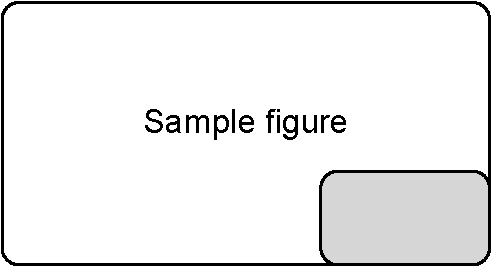
\includegraphics[scale=0.5]{sample-figure}
  \caption{Sample figure}
  \label{fig1:../Figures/sample}
\end{figure}

\subsubsection{Subsubsection}

Integer eleifend quam et odio iaculis, at elementum augue aliquam.
Ut eu nibh nec urna finibus semper fermentum id purus.
Aliquam eu sollicitudin libero.
Cras viverra elit congue erat pulvinar, vitae vehicula tortor interdum.
Aliquam commodo mi sapien, ullamcorper egestas velit tempor nec.
Quisque sapien velit, fringilla non vulputate nec, lacinia in dui.
Nam vestibulum volutpat ante, eu sodales enim tincidunt vel.
Ut mollis elit quis bibendum eleifend.
In laoreet tortor non odio ultrices mollis.
Curabitur volutpat et risus quis fermentum.
Morbi laoreet ligula eget orci consectetur, in dictum ipsum efficitur.
Mauris nec neque ultricies, efficitur elit id, hendrerit nibh.
Interdum et malesuada fames ac ante ipsum primis in faucibus.

\paragraph{Paragraph}

Nulla scelerisque id lectus a luctus.
Curabitur quis dolor maximus, maximus erat ut, placerat justo.
Donec auctor purus a lacus molestie maximus.
Etiam porta ligula a quam mollis efficitur.
Quisque vel sapien iaculis, pellentesque lorem nec, hendrerit lectus.
Vestibulum egestas congue euismod.
Praesent a tristique massa.
Aliquam eget ante elit.
Phasellus eget metus mi.
Fusce nec rutrum mi.
Pellentesque eu congue mi.
Fusce eu ullamcorper est.

\section{Background}

Refer to \verb|acmart.pdf| \cite{veytsmanlatex} (\url{https://www.ctan.org/pkg/acmart}, \url{http://www.acm.org/publications/proceedings-template}) for additional examples and instructions.

\subsection{Subsection}

Lorem ipsum dolor sit amet, consectetur adipiscing elit.
Sed aliquam nisl turpis, sit amet mollis leo accumsan vel.
Donec semper turpis dui, a porttitor lorem tincidunt id.
Phasellus gravida, purus non faucibus euismod, lectus tortor maximus elit, vestibulum lobortis purus turpis non urna.
Fusce feugiat lectus ut massa molestie, non interdum augue porta.
Nunc dapibus odio nec neque cursus, ut lacinia velit rutrum.
Duis tempor nulla velit, sed pellentesque nunc imperdiet ut.
Phasellus eget hendrerit neque.
Suspendisse aliquet nulla id sem aliquam aliquam sed a orci.
Duis sem est, hendrerit nec porttitor sit amet, maximus sed nulla.
Suspendisse et dictum massa.
Morbi non diam nec orci sodales eleifend.
Etiam eget finibus purus, a malesuada ipsum.
Nullam ac nisi nec elit faucibus aliquet.
Nulla feugiat velit sed sodales eleifend.
Donec orci nulla, viverra et mi in, sagittis egestas urna.

\begin{figure}[htbp]
  \centering
  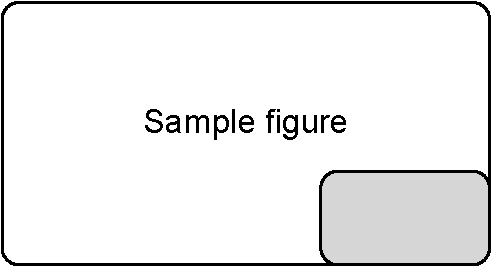
\includegraphics[scale=0.5]{sample-figure}
  \caption{Sample figure}
  \Description{Sample figure description.}
  \label{fig2:../Figures/sample}
\end{figure}

\subsubsection{Subsubsection}

Integer eleifend quam et odio iaculis, at elementum augue aliquam.
Ut eu nibh nec urna finibus semper fermentum id purus.
Aliquam eu sollicitudin libero.
Cras viverra elit congue erat pulvinar, vitae vehicula tortor interdum.
Aliquam commodo mi sapien, ullamcorper egestas velit tempor nec.
Quisque sapien velit, fringilla non vulputate nec, lacinia in dui.
Nam vestibulum volutpat ante, eu sodales enim tincidunt vel.
Ut mollis elit quis bibendum eleifend.
In laoreet tortor non odio ultrices mollis.
Curabitur volutpat et risus quis fermentum.
Morbi laoreet ligula eget orci consectetur, in dictum ipsum efficitur.
Mauris nec neque ultricies, efficitur elit id, hendrerit nibh.
Interdum et malesuada fames ac ante ipsum primis in faucibus.

\paragraph{Paragraph}

Nulla scelerisque id lectus a luctus.
Curabitur quis dolor maximus, maximus erat ut, placerat justo.
Donec auctor purus a lacus molestie maximus.
Etiam porta ligula a quam mollis efficitur.
Quisque vel sapien iaculis, pellentesque lorem nec, hendrerit lectus.
Vestibulum egestas congue euismod.
Praesent a tristique massa.
Aliquam eget ante elit.
Phasellus eget metus mi.
Fusce nec rutrum mi.
Pellentesque eu congue mi.
Fusce eu ullamcorper est.

\section{Proposal}

Refer to \verb|acmart.pdf| \cite{veytsmanlatex} (\url{https://www.ctan.org/pkg/acmart}, \url{http://www.acm.org/publications/proceedings-template}) for additional examples and instructions.

\subsection{Subsection}

Lorem ipsum dolor sit amet, consectetur adipiscing elit.
Sed aliquam nisl turpis, sit amet mollis leo accumsan vel.
Donec semper turpis dui, a porttitor lorem tincidunt id.
Phasellus gravida, purus non faucibus euismod, lectus tortor maximus elit, vestibulum lobortis purus turpis non urna.
Fusce feugiat lectus ut massa molestie, non interdum augue porta.
Nunc dapibus odio nec neque cursus, ut lacinia velit rutrum.
Duis tempor nulla velit, sed pellentesque nunc imperdiet ut.
Phasellus eget hendrerit neque.
Suspendisse aliquet nulla id sem aliquam aliquam sed a orci.
Duis sem est, hendrerit nec porttitor sit amet, maximus sed nulla.
Suspendisse et dictum massa.
Morbi non diam nec orci sodales eleifend.
Etiam eget finibus purus, a malesuada ipsum.
Nullam ac nisi nec elit faucibus aliquet.
Nulla feugiat velit sed sodales eleifend.
Donec orci nulla, viverra et mi in, sagittis egestas urna.

\begin{figure}[htbp]
  \centering
  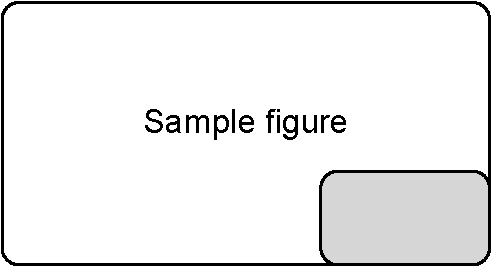
\includegraphics[scale=0.5]{sample-figure}
  \caption{Sample figure}
  \Description{Sample figure description.}
  \label{fig3:../Figures/sample}
\end{figure}

\subsubsection{Subsubsection}

Integer eleifend quam et odio iaculis, at elementum augue aliquam.
Ut eu nibh nec urna finibus semper fermentum id purus.
Aliquam eu sollicitudin libero.
Cras viverra elit congue erat pulvinar, vitae vehicula tortor interdum.
Aliquam commodo mi sapien, ullamcorper egestas velit tempor nec.
Quisque sapien velit, fringilla non vulputate nec, lacinia in dui.
Nam vestibulum volutpat ante, eu sodales enim tincidunt vel.
Ut mollis elit quis bibendum eleifend.
In laoreet tortor non odio ultrices mollis.
Curabitur volutpat et risus quis fermentum.
Morbi laoreet ligula eget orci consectetur, in dictum ipsum efficitur.
Mauris nec neque ultricies, efficitur elit id, hendrerit nibh.
Interdum et malesuada fames ac ante ipsum primis in faucibus.

\paragraph{Paragraph}

Nulla scelerisque id lectus a luctus.
Curabitur quis dolor maximus, maximus erat ut, placerat justo.
Donec auctor purus a lacus molestie maximus.
Etiam porta ligula a quam mollis efficitur.
Quisque vel sapien iaculis, pellentesque lorem nec, hendrerit lectus.
Vestibulum egestas congue euismod.
Praesent a tristique massa.
Aliquam eget ante elit.
Phasellus eget metus mi.
Fusce nec rutrum mi.
Pellentesque eu congue mi.
Fusce eu ullamcorper est.

\section{Results}

Refer to \verb|acmart.pdf| \cite{veytsmanlatex} (\url{https://www.ctan.org/pkg/acmart}, \url{http://www.acm.org/publications/proceedings-template}) for additional examples and instructions.

\subsection{Subsection}

Lorem ipsum dolor sit amet, consectetur adipiscing elit.
Sed aliquam nisl turpis, sit amet mollis leo accumsan vel.
Donec semper turpis dui, a porttitor lorem tincidunt id.
Phasellus gravida, purus non faucibus euismod, lectus tortor maximus elit, vestibulum lobortis purus turpis non urna.
Fusce feugiat lectus ut massa molestie, non interdum augue porta.
Nunc dapibus odio nec neque cursus, ut lacinia velit rutrum.
Duis tempor nulla velit, sed pellentesque nunc imperdiet ut.
Phasellus eget hendrerit neque.
Suspendisse aliquet nulla id sem aliquam aliquam sed a orci.
Duis sem est, hendrerit nec porttitor sit amet, maximus sed nulla.
Suspendisse et dictum massa.
Morbi non diam nec orci sodales eleifend.
Etiam eget finibus purus, a malesuada ipsum.
Nullam ac nisi nec elit faucibus aliquet.
Nulla feugiat velit sed sodales eleifend.
Donec orci nulla, viverra et mi in, sagittis egestas urna.

\begin{figure}[htbp]
  \centering
  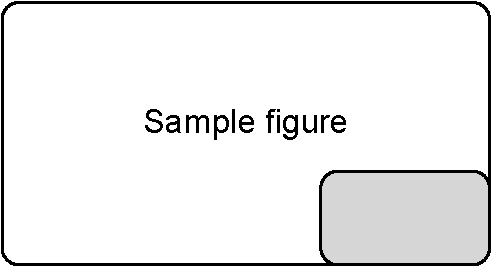
\includegraphics[scale=0.5]{sample-figure}
  \caption{Sample figure}
  \label{fig4:../Figures/sample}
\end{figure}

\subsubsection{Subsubsection}

Integer eleifend quam et odio iaculis, at elementum augue aliquam.
Ut eu nibh nec urna finibus semper fermentum id purus.
Aliquam eu sollicitudin libero.
Cras viverra elit congue erat pulvinar, vitae vehicula tortor interdum.
Aliquam commodo mi sapien, ullamcorper egestas velit tempor nec.
Quisque sapien velit, fringilla non vulputate nec, lacinia in dui.
Nam vestibulum volutpat ante, eu sodales enim tincidunt vel.
Ut mollis elit quis bibendum eleifend.
In laoreet tortor non odio ultrices mollis.
Curabitur volutpat et risus quis fermentum.
Morbi laoreet ligula eget orci consectetur, in dictum ipsum efficitur.
Mauris nec neque ultricies, efficitur elit id, hendrerit nibh.
Interdum et malesuada fames ac ante ipsum primis in faucibus.

\paragraph{Paragraph}

Nulla scelerisque id lectus a luctus.
Curabitur quis dolor maximus, maximus erat ut, placerat justo.
Donec auctor purus a lacus molestie maximus.
Etiam porta ligula a quam mollis efficitur.
Quisque vel sapien iaculis, pellentesque lorem nec, hendrerit lectus.
Vestibulum egestas congue euismod.
Praesent a tristique massa.
Aliquam eget ante elit.
Phasellus eget metus mi.
Fusce nec rutrum mi.
Pellentesque eu congue mi.
Fusce eu ullamcorper est.

\section{Conclusions}

Refer to \verb|acmart.pdf| \cite{veytsmanlatex} (\url{https://www.ctan.org/pkg/acmart}, \url{http://www.acm.org/publications/proceedings-template}) for additional examples and instructions.

\subsection{Subsection}

Lorem ipsum dolor sit amet, consectetur adipiscing elit.
Sed aliquam nisl turpis, sit amet mollis leo accumsan vel.
Donec semper turpis dui, a porttitor lorem tincidunt id.
Phasellus gravida, purus non faucibus euismod, lectus tortor maximus elit, vestibulum lobortis purus turpis non urna.
Fusce feugiat lectus ut massa molestie, non interdum augue porta.
Nunc dapibus odio nec neque cursus, ut lacinia velit rutrum.
Duis tempor nulla velit, sed pellentesque nunc imperdiet ut.
Phasellus eget hendrerit neque.
Suspendisse aliquet nulla id sem aliquam aliquam sed a orci.
Duis sem est, hendrerit nec porttitor sit amet, maximus sed nulla.
Suspendisse et dictum massa.
Morbi non diam nec orci sodales eleifend.
Etiam eget finibus purus, a malesuada ipsum.
Nullam ac nisi nec elit faucibus aliquet.
Nulla feugiat velit sed sodales eleifend.
Donec orci nulla, viverra et mi in, sagittis egestas urna.

\begin{figure}[htbp]
  \centering
  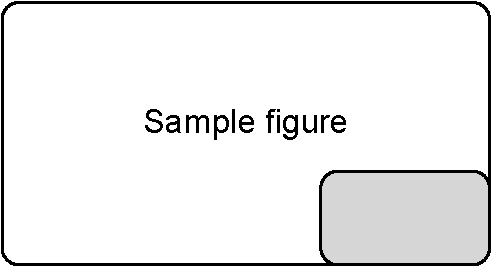
\includegraphics[scale=0.5]{sample-figure}
  \caption{Sample figure}
  \Description{Sample figure description.}
  \label{fig5:../Figures/sample}
\end{figure}

\subsubsection{Subsubsection}

Integer eleifend quam et odio iaculis, at elementum augue aliquam.
Ut eu nibh nec urna finibus semper fermentum id purus.
Aliquam eu sollicitudin libero.
Cras viverra elit congue erat pulvinar, vitae vehicula tortor interdum.
Aliquam commodo mi sapien, ullamcorper egestas velit tempor nec.
Quisque sapien velit, fringilla non vulputate nec, lacinia in dui.
Nam vestibulum volutpat ante, eu sodales enim tincidunt vel.
Ut mollis elit quis bibendum eleifend.
In laoreet tortor non odio ultrices mollis.
Curabitur volutpat et risus quis fermentum.
Morbi laoreet ligula eget orci consectetur, in dictum ipsum efficitur.
Mauris nec neque ultricies, efficitur elit id, hendrerit nibh.
Interdum et malesuada fames ac ante ipsum primis in faucibus.

\paragraph{Paragraph}

Nulla scelerisque id lectus a luctus.
Curabitur quis dolor maximus, maximus erat ut, placerat justo.
Donec auctor purus a lacus molestie maximus.
Etiam porta ligula a quam mollis efficitur.
Quisque vel sapien iaculis, pellentesque lorem nec, hendrerit lectus.
Vestibulum egestas congue euismod.
Praesent a tristique massa.
Aliquam eget ante elit.
Phasellus eget metus mi.
Fusce nec rutrum mi.
Pellentesque eu congue mi.
Fusce eu ullamcorper est.


\bibliographystyle{acm}
\bibliography{sigproc}

\end{document}
